\documentclass[border=5pt]{standalone}
\usepackage{tikz}
\usepackage{xcolor}
\usetikzlibrary{calc,shadows.blur}

% J2 - Green metallic shaft
\begin{document}
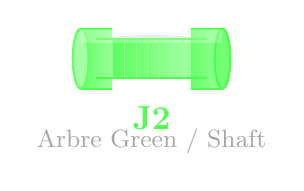
\begin{tikzpicture}

% Shadow
\fill[gray!20,blur shadow={shadow blur steps=5}] (1,0.15) ellipse (0.9 and 0.15);

% Shaft body with stepped profile
\fill[left color=green!70, right color=green!30, middle color=green!50]
  (0.3,-0.25) rectangle (1.7,0.25);

% Stepped shoulder left
\fill[left color=green!60, right color=green!40]
  (0.1,-0.38) rectangle (0.5,0.38);

% Stepped shoulder right
\fill[left color=green!60, right color=green!40]
  (1.5,-0.38) rectangle (1.9,0.38);

% End caps
\fill[green!35] (0.1,0) ellipse (0.1 and 0.38);
\draw[green!60,thick] (0.1,0) ellipse (0.1 and 0.38);
\fill[green!55] (1.9,0) ellipse (0.1 and 0.38);
\draw[green!70,thick] (1.9,0) ellipse (0.1 and 0.38);

% Outlines
\draw[green!70, line width=0.8pt]
  (0.3,-0.25)--(1.7,-0.25) (0.3,0.25)--(1.7,0.25);
\draw[green!70, line width=0.8pt]
  (0.1,-0.38)--(0.5,-0.38) (0.1,0.38)--(0.5,0.38);
\draw[green!70, line width=0.8pt]
  (1.5,-0.38)--(1.9,-0.38) (1.5,0.38)--(1.9,0.38);

% Highlight
\fill[white,opacity=0.25] (0.1,0.2) rectangle (1.9,0.38);

% Thread lines on main shaft
\foreach \x in {0.5,0.65,0.8,0.95,1.1,1.25,1.4}{
  \draw[green!40,very thin] (\x,-0.25)--(\x,0.25);
}

% Label
\node[font=\bfseries\large, text=green!70] at (1.0,-0.75) {J2};
\node[font=\small, text=gray!70] at (1.0,-1.05) {Arbre Green / Shaft};

\end{tikzpicture}
\end{document}
